\documentclass{beamer}
%\documentclass{article}
%\usepackage{beamerarticle}
%\pagestyle{plain}
\newcommand{\bfX}{{\mbox{{\bf X}}}}
\newcommand{\bfR}{{\mbox{{\bf R}}}}

\usepackage{amssymb}
\usepackage{amsmath}
\newcommand\reals{\ensuremath{\mathbb{R}}}
%\newcommand{\bfX}{{\mbox{{\bf X}}}}
\newcommand{\bfY}{{\mbox{{\bf Y}}}}
\DeclareFontShape{OT1}{cmtt}{bx}{n}{
  <5><6><7><8><9><10><10.95><12><14.4><17.28><20.74><24.88>cmttb10}{}



\listfiles

\renewcommand\emptyset{\varnothing}
%\renewcommand\cdot{\mathop{\raise2pt\hbox{$\bullet$}}}
\renewcommand\cdot{\mathop{\raise-1pt\hbox{$^{_\bullet}$}}}

\renewcommand\today{November 21, 2017}
\title[cars.com]{
Data scraping, ingestation, and modeling: bringing data from cars.com into the intro stats class}
\author{Nicholas J. Horton}
\institute{{\large Department of Mathematics and Statistics \\Amherst College, Amherst, MA, USA}}
\date{CAUSE webinar, \today}


\mode<presentation>
{
  \usetheme{Warsaw}
  %\usetheme{Copenhagen}
  % or ...

  %\setbeamercovered{transparent}
  % or whatever (possibly just delete it)
}

\AtBeginSubsection[]
{
  %\begin{frame}<beamer>
    %\frametitle{Outline}
    %\tableofcontents[currentsection,currentsubsection]
  %\end{frame}
}



\begin{document}
\frame{\titlepage
nhorton@amherst.edu \\
http://nhorton.people.amherst.edu, https://github.com/Amherst-Statistics/Cars-Scraping-Webinar}


\frame{
\frametitle{Thanks and acknowledgements}
\begin{itemize}
\item Danny Kaplan (for the original idea)
\item Project MOSAIC: Danny Kaplan (Macalester College), Randy Pruim (Calvin College), Ben Baumer (Smith College), and Johanna Hardin (Pomona College)
\item NSF \# 0920350
\end{itemize}
}

\frame{
\frametitle{Goal}
\begin{itemize}
\item I will describe a classroom activity where pairs of students hand scrape data from cars.com, ingest these data into R, then carry out analyses of the relationships between price, mileage, and model year for a selected type of car. 
\item This early in the semester activity can help illustrate the statistical problem solving process. 
\item The ``Less Volume, More Creativity" approach utilized by the mosaic package facilitates the analysis with a minimal amount of syntax. 
\item Key concepts that are introduced and reinforced including data ingestion, multivariate thinking through graphical visualizations, and regression modeling. 
\item Extensions and additional use of the dataset will be discussed along with potential pitfalls.
\end{itemize}
}

\frame{
\frametitle{Cars, cars, and more cars}
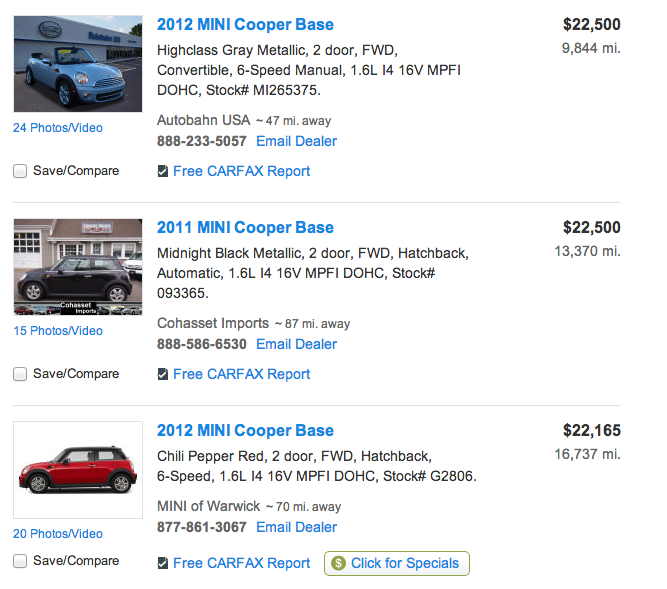
\includegraphics[scale=0.52]{cars.png}
}

\frame{
\frametitle{Questions?}
\begin{itemize}
\item How much do cars cost?
\item How much do car prices vary?
\item How are car prices associated with mileage?
\item How are car prices associated with age?
\item How quickly do new cars depreciate?
\item How much does it cost for a car to drive a mile?
\end{itemize}
}

\frame{
\frametitle{revised GAISE College report}

\includegraphics[scale=0.28]{gaise}}

\frame{
\frametitle{revised GAISE College Report (2016)}
\begin{enumerate}
\item Teach statistical thinking.
\begin{itemize}
\item Teach statistics as an investigative process of problem-solving and decision-making.
\item Give students experience with \emph{multivariable thinking}.
\end{itemize}
\item Focus on conceptual understanding.
\item Integrate real data with a context and purpose.
\item Foster active learning.
\item Use technology to explore concepts and analyze data.
\item Use assessments to improve and evaluate student learning.
\end{enumerate}
}

\frame{
\frametitle{Motivation for multivariate thinking}
\begin{itemize}
\item How much do cars cost?
\item How much do car prices vary?
\item How are car prices associated with mileage?
\item How are car prices associated with age?
\item How quickly do new cars depreciate?
\item How much does it cost for a car to drive a mile?
\end{itemize}
}

\frame{
\frametitle{Closing thoughts}
\begin{itemize}
\item Ensure that students see multivariate examples early and often
\item Ensure that students use real tools
\item Once they have some experience with ``tame data", have them ingest their own
\item Motivate automated data scraping procedures
\item Practice composing and answering questions with data
\end{itemize}
}

\frame{\titlepage
nhorton@amherst.edu \\
http://nhorton.people.amherst.edu, https://github.com/Amherst-Statistics/Cars-Scraping-Webinar}

\end{document}
